\section{Challenge: Final Use Cases and Further Functionality}
\label{sec:challenge_final_use_cases_and_further_functionality}

\subsection{Challenge AddMissingFunctionalitiesToCarRentalCLI}
\label{subsec:challenge_addmissingfunctionalitiestocarrentalcli}

\subsubsection*{Implement Use Cases}
Two use cases are missing in the CarRentalCLI program.

The first use case is to cancel an already existing rental.

The implementation process is quite similar to the already implemented use cases.
\texttt{CarRentalCLI.go} holds the CLI commands.
By adding "cancel" to the commands array, the command can be used in the CLI.
The command calls the \texttt{CancelRentalAction} function, taking the operations as input.

\texttt{CancelRentalAction} prints "Cancel a rental" and collects the rentalID from the user.
The rental is then cancelled by calling \texttt{CancelRental}, taking the rentalID as input.

\texttt{CancelRental} verifies the rentalID by checking if it exists. \hfill \linebreak
It then calls \texttt{DeleteRental(rentalID)} to delete the rental.
The \texttt{DeleteRental} function located in the repository removes the rental from the repository, then saves the data to the yaml files.

If everything ran successfully, a success message is printed to the user containing the removed rentalID.
If an error happens during runtime, the application exits safely.

To test the function, a new file called \texttt{CancelRentalOperation\_test.go} is created.
It uses the already implemented \texttt{SetupMockCarRentalRepository} function from \hfill \linebreak \texttt{CarRentalRepository\_test.go} to create a mock repository.

The function running the tests is similar to the already implemented test function from \texttt{CarRentalRepository\_test.go} besides the test cases.
The test cases only contain the rentalID as parameter, since it is the only imput needed to delete a rental.

Two test cases are implemented:
The first test case is non conflicting and deletes the already existing first rental.
The second test case is built to fail by wanting to delete a non existing rental.

Both tests succeed as shown in \autoref{fig:carRentalCLI_challenge_successfulCancellationOfRentalTest}.

\begin{figure}
    \centering
    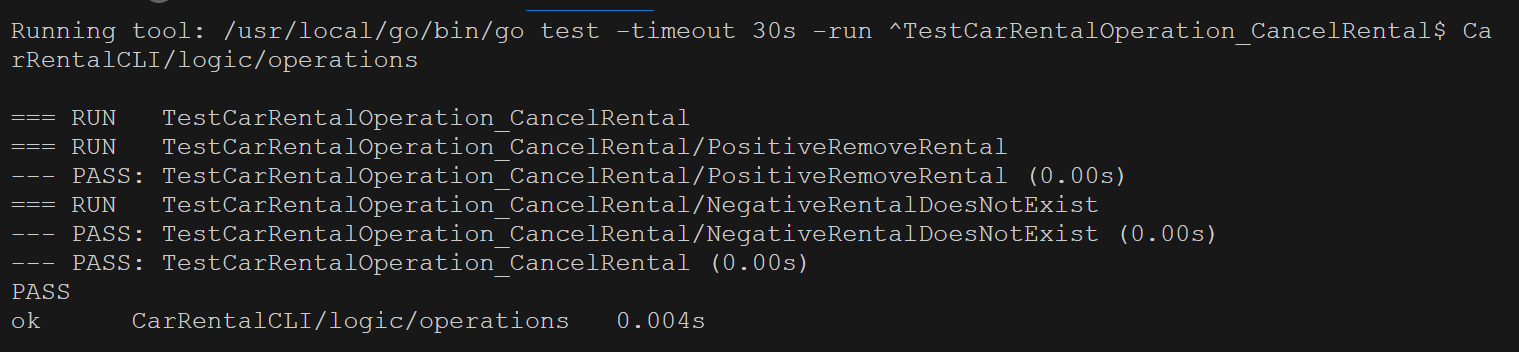
\includegraphics[width=0.8\textwidth]{figures/goLang/carRental/carRentalCLI/challenge/carRentalCLI_challenge_successfulCancellationOfRentalTest.png}
    \caption{Successful Tests of the newly implemented CancelRental Function}
    \label{fig:carRentalCLI_challenge_successfulCancellationOfRentalTest}
\end{figure}

%//TODO implement second use case
